As concluded from the theoretical considerations discussed in the introduction, it 
is hypothesized that the period of oscillation $T$ is independent of the mass $m$, 
the initial angular amplitude $\theta_0$, and is related to the length of the string 
by Eq.(\ref{period}). Figure \ref{length_period} plots the estimated period of oscillation, 
optimized by \texttt{curve\_fit} over the first 100 time steps, against their respective 
lengths $\ell$ for the five data sets with a fixed mass $m = 0.1\text{kg}$ and fixed 
initial angular amplitude $\theta_0 = 0.22\text{rads}$. The lengths used lie in the domain 
$(0.075\text{m}, 0.20\text{m})$ with the associated periods lying in the domain 
$(0.65\text{s}, 1.00\text{s})$. These data points are then fitted with a functional form 
$T = A\sqrt{\ell} = A\sqrt{L + D}$, with the proportionality constant taking on a value of 
$A = (1.96\pm 0.09)[\text{s}/\sqrt{\text{m}}]$, a value which certainly has magnitude 
comparable to the hypothesized proportionality constant $A = 2$. The uncertainty propagation 
of $A$ is done using the covariance matrix provided by \texttt{curve\_fit}. The optimized 
fit carries a goodness of fit estimation of $\chi^2 = 1.85$; this indicates a strong 
correlation between the collected data and fitted functional form. Up to uncertainty, 
the expected value of the constant of proportionality, $A = 2 [\text{s}/\sqrt{\text{m}}]$, 
and the computed value, $A = (1.96 \pm 0.09)[\text{s}/\sqrt{\text{m}}]$, are equal in value, 
and thus the validity of Eq.(\ref{period}) is concluded.


\begin{figure}[H]
\centering
\begin{subfigure}[t]{0.5\textwidth}
  \centering
  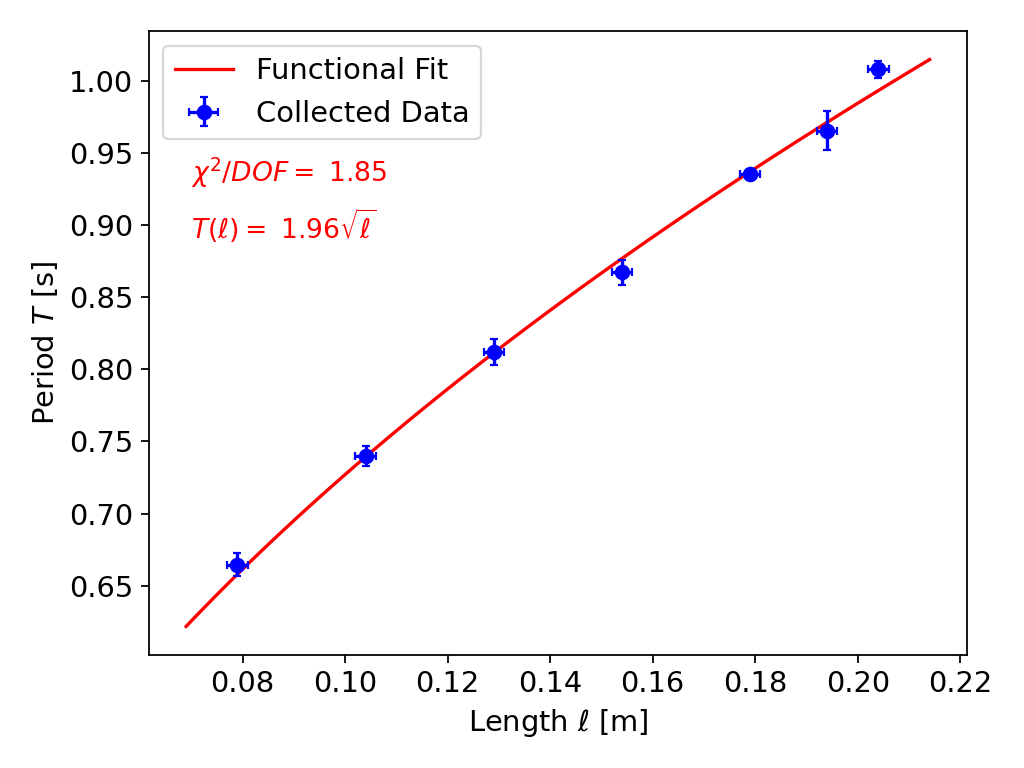
\includegraphics[width=1\linewidth]{Plots/length_vs_period.png}
  \caption{\small{Length versus estimated period of oscillation.}}
  \label{length_period}
\end{subfigure}%
\begin{subfigure}[t]{0.5\textwidth}
  \centering
  \includegraphics[width=1\linewidth]{Plots/length_vs_period_residual.png}
  \caption{\small{Residuals of collected data versus optimized fit.}}
  \label{length_period_residual}
\end{subfigure}
\caption{\small{(Left) A plot of the pendulum length versus estimated period of oscillation of the collected data sets with fixed mass $m = 0.10\text{kg}$ and initial angle $\theta_0 = 0.22\text{rad}$. This data is approximated with a functional fit of the form $T(\ell) = A\sqrt{\ell}$, where the proportionality constant $A$ was optimized to take on a value of $A = (1.96\pm 0.09)\frac{\text{s}}{\sqrt{\text{m}}}$. Further, a goodness of fit estimate takes on a value of $\chi^2 = 1.94$, indicating a strong correlation. (Right) A plot of the residual values between the collected data and the associated functional forms.}}
\end{figure}


To verify that the period of oscillation is independent of the masses being used, 
Figure \ref{mass_period} is generated, plotting the estimated periods for each associated 
weight while leaving $L = 0.1\text{m}$ and $\theta_0 = 0.22\text{rad}$ fixed. These data 
points are plotted alongside the constant function which takes on a value equal to that of 
the average period of the five data sets under consideration. There is indeed significant 
deviation between each singular value of $T$ and the average value of $T$, however these 
deviations are at least an order of magnitude smaller than the magnitude of the periods 
themselves. Further discussion on these deviations is included in the uncertainty analysis 
section of this report. Observing the differentiation between the values of $T$ for subsequent 
masses, it is rather clear that there is no suitable correlation between the mass and the 
period other than their mutual independence. Indeed if there were a relation, the period 
would be either increasing or decreasing with an increase in mass, neither trend of which 
accurately describes the behaviour present in Figure \ref{mass_period}. As such, this data 
allows for conclusivity; the period of oscillation $T$ is independent of the mass $m$ of the 
weights being used. \\[0.20cm]


\begin{figure}[H]
\centering
\begin{subfigure}[t]{0.5\textwidth}
  \centering
  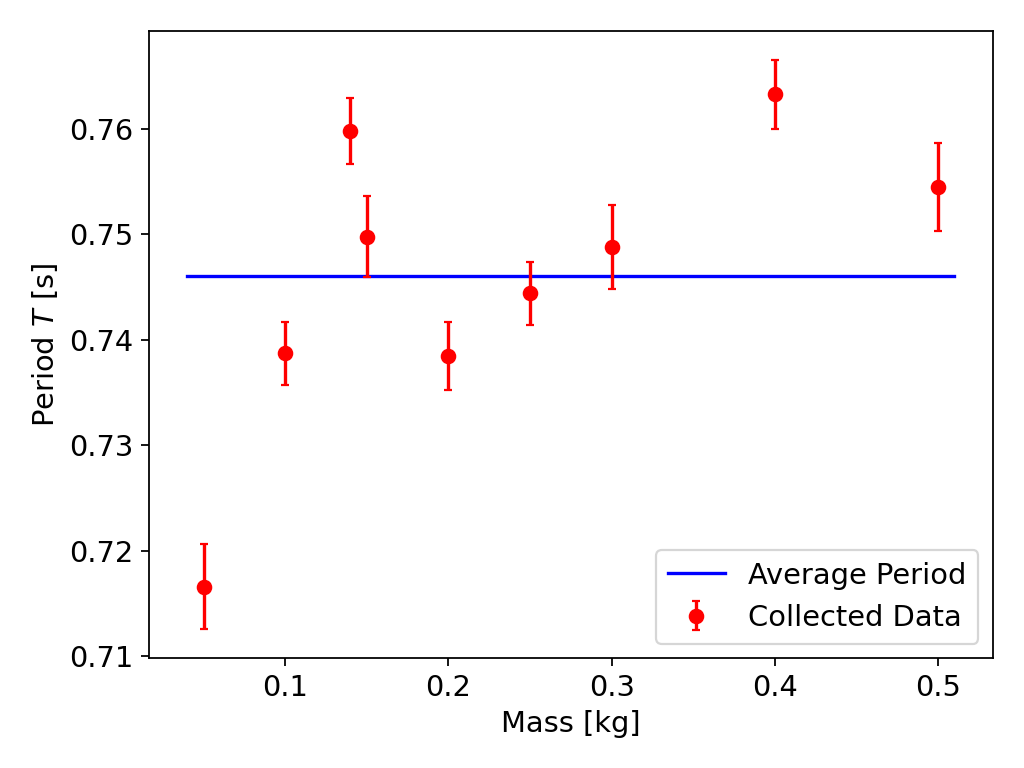
\includegraphics[width=1\textwidth]{Plots/mass_vs_period.png}
  \caption{\small{Mass versus estimated period}}
  \label{mass_period}
\end{subfigure}%
\begin{subfigure}[t]{.5\textwidth}
  \centering
  \includegraphics[width=\textwidth]{Plots/amplitude_vs_period.png}
  \caption{\small{Initial angular amplitude versus estimated period}}
  \label{amplitude_period}
\end{subfigure}
\caption{\small{(Left) A plot of the mass versus estimated period of oscillation of the collected data sets with fixed length $L = 0.10\text{m}$ and initial angle $\theta_0 = 0.22\text{rad}$. These points are plotted alongside the constant function of magnitude equal to the average value of the estimated periods. (Right) A plot of the initial angular amplitude versus estimated period of oscillation of the collected data sets with fixed length $L = 0.10\text{m}$ and mass $m = 0.05\text{kg}$. These points are plotted alongside the constant function of magnitude equal to the average value of the estimated periods.}}
\end{figure}

Finally, to verify the independence of the period $T$ on the initial angular amplitude 
$\theta_0$, Figure \ref{amplitude_period} plots the estimated period of oscillation 
against the initial angular amplitude that each data set underwent. The average value of 
the estimated periods is plotted alongside the data points. In an effort to truly display 
the existance of the small angle approximation, eight (8) distinct data sets have been 
recorder, five of which take on initial angular amplitude less that $0.25\text{rads} \approx 15^o$. 
As is clearly evident in the generated plots, the estimated period takes on highly consistent 
values for the first five data sets -- the collection whose initial amplitude is sufficiently 
small. In fact, up to uncertainty, the first five estimated periods are equal. Further increasing 
the initial amplitude, however, results in an increase in the period of oscillation. This trend 
remains consistent for all of the plot points whose initial angular amplitude exceeds $0.25\text{rads}$. 
Hence, it is appropriate to conclude that the period of oscillation is independent of the initial 
amplitude, so long as the initial amplitude is sufficiently small.

